\documentclass[12pt]{article}
\pagestyle{empty}
\usepackage{graphicx}
\usepackage{subcaption}
\usepackage{amsmath}
\usepackage{amsfonts}

\title{Stabilized FEM Homework 1}
\author{Truman Ellis}
\date{}

\begin{document}
\section*{Problem 8.1}
\paragraph{b)}
Cross sections of $g'_e(x,y)$ at $y=0.5$ for $u=h^e=1$.
\begin{figure}[h!]
\centering
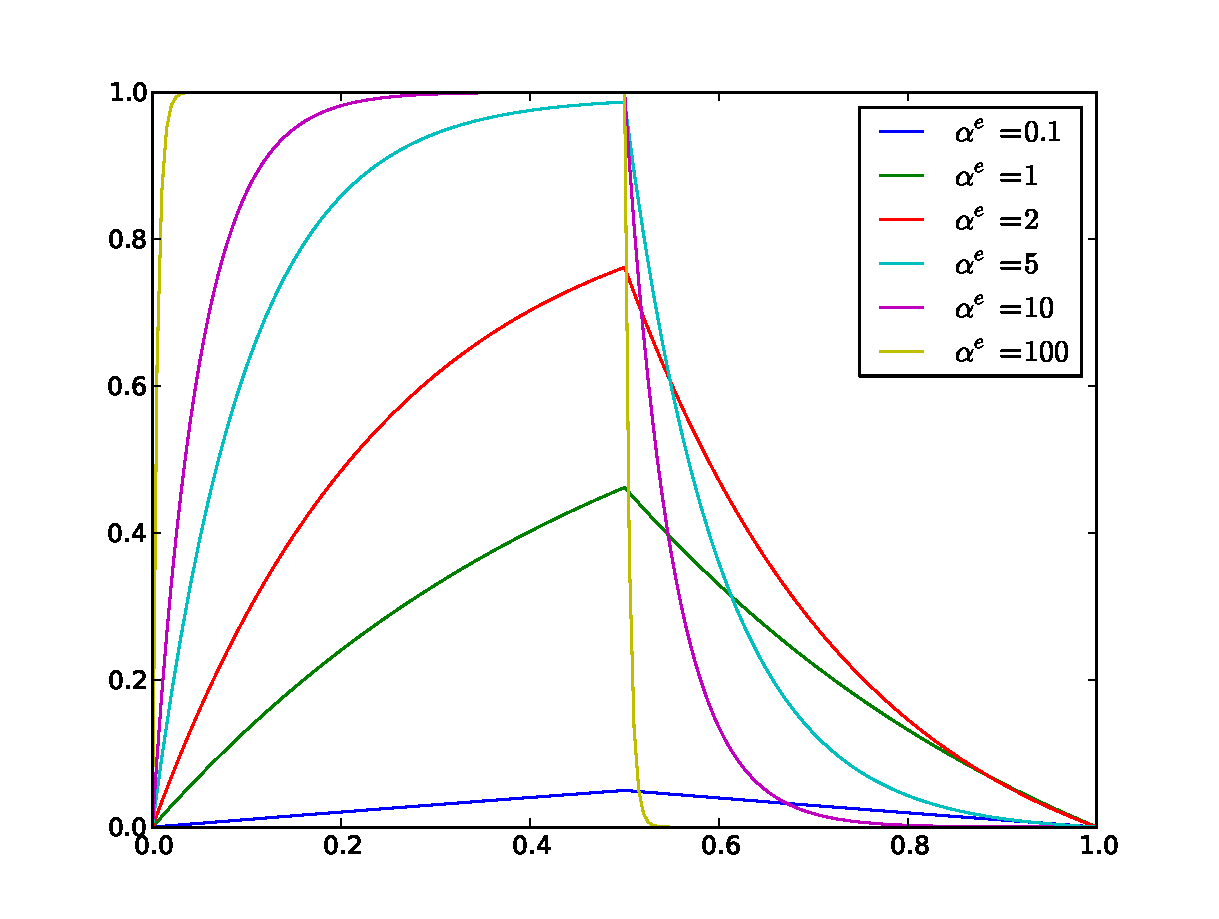
\includegraphics[width=0.8\textwidth]{lines.pdf}
\end{figure}


\clearpage
\newpage
\paragraph{c)}
Elevation plots of $g'_e(x,y)$ for $u=h^e=1$.
\begin{figure}[h!]
\centering
\begin{subfigure}[c]{0.3\textwidth}
\centering
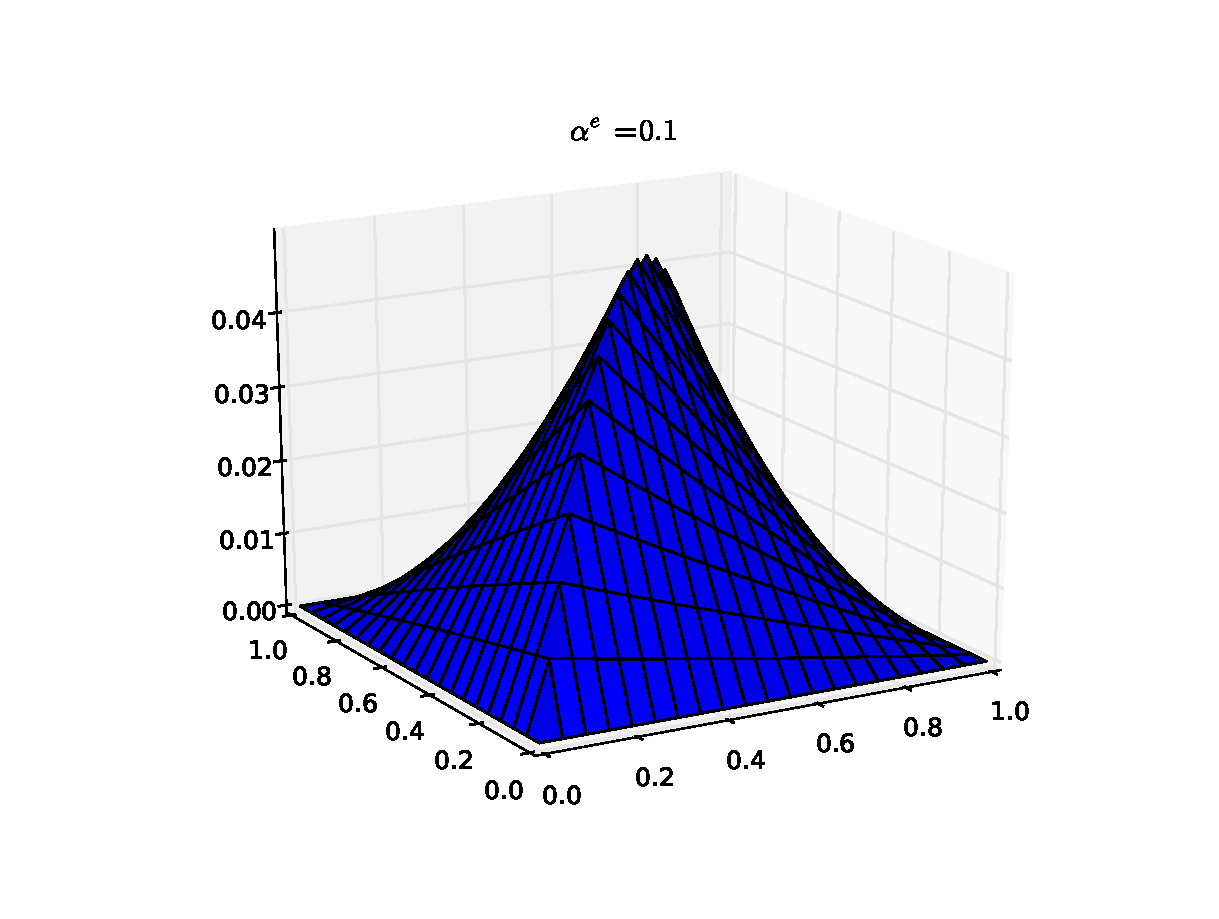
\includegraphics[width=\textwidth]{surf1e-1.pdf}
\caption{One}
\end{subfigure}
\end{figure}
% \begin{figure}[h!]
% \centering
% \mbox{\subfigure{
% 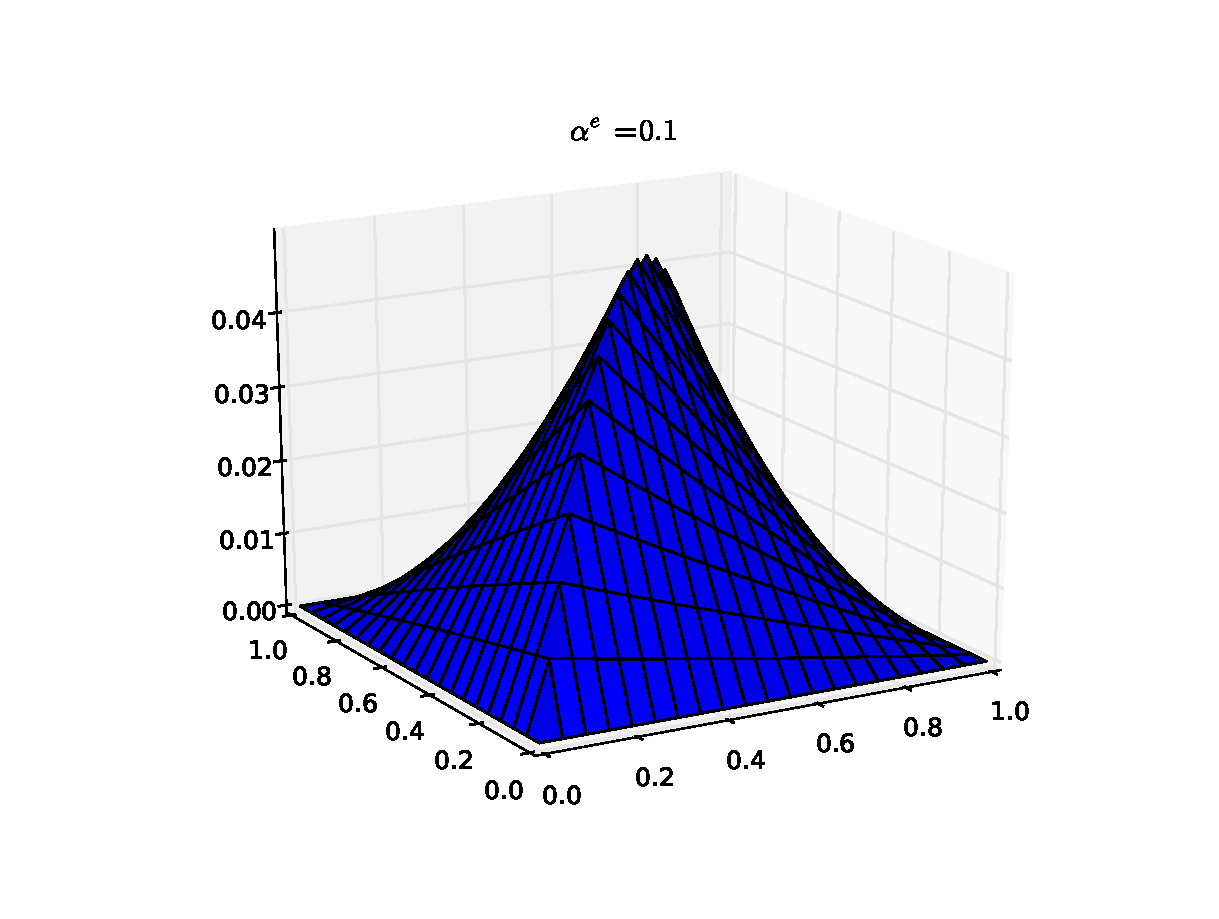
\includegraphics[width=0.45\textwidth]{surf1e-1.pdf}
% }
% \subfigure{
% 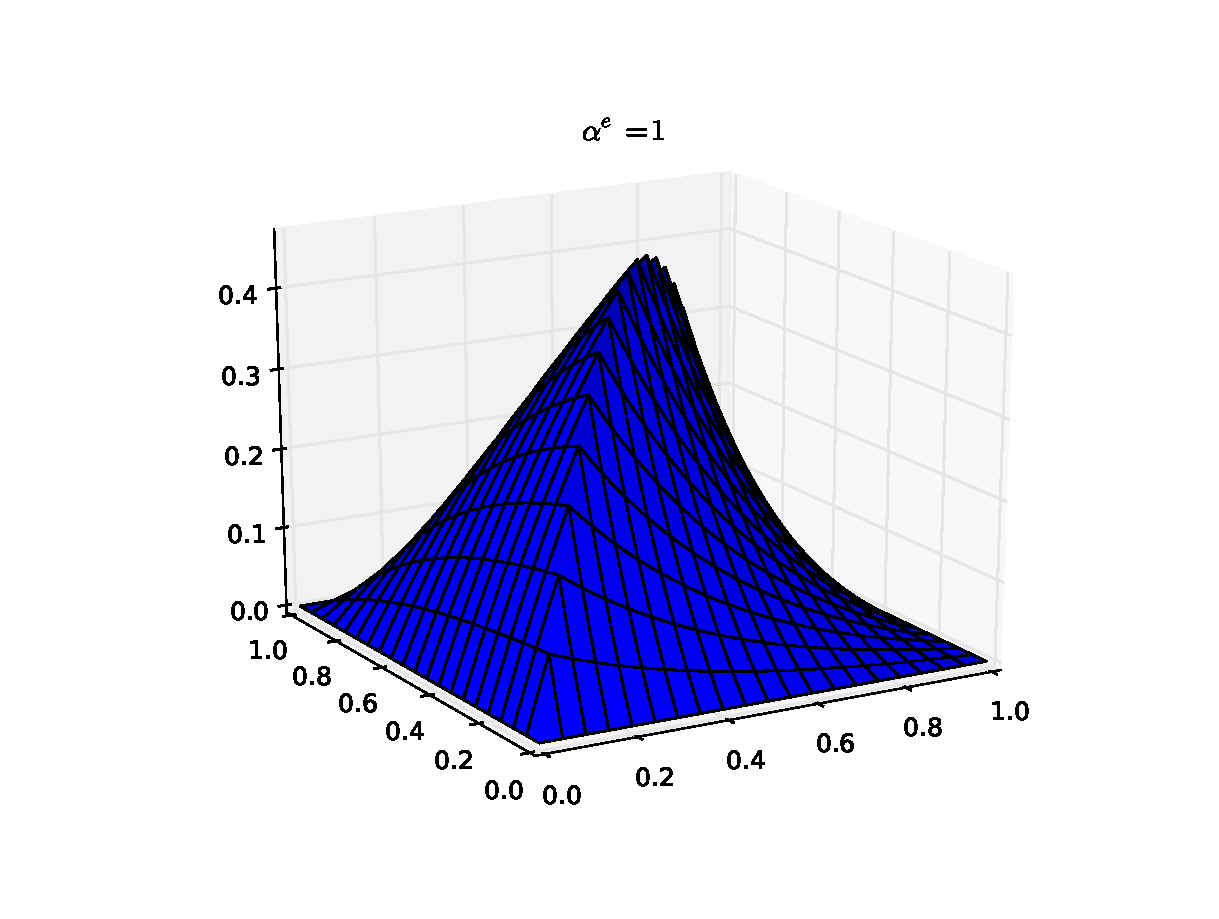
\includegraphics[width=0.45\textwidth]{surf1e0.pdf}
% }}
% \mbox{\subfigure{
% 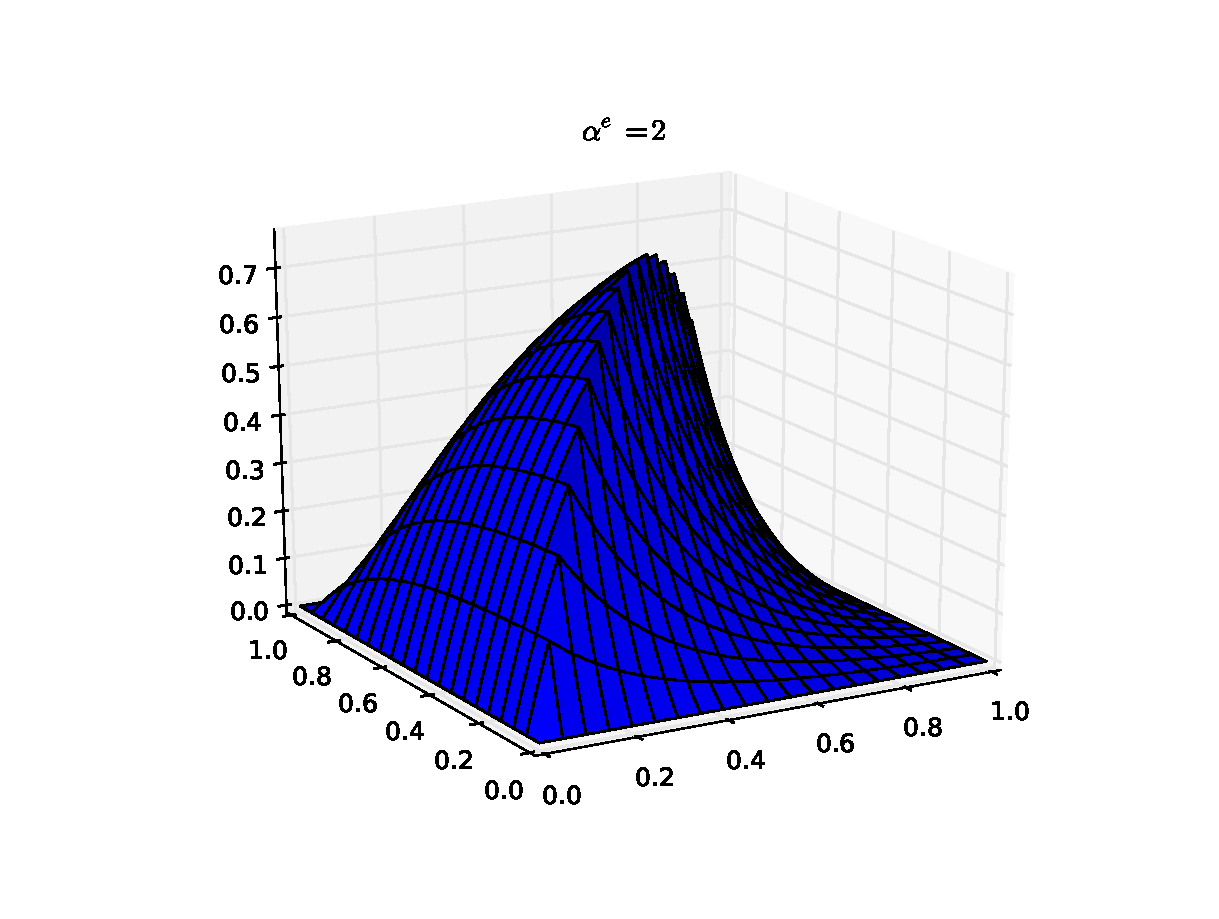
\includegraphics[width=0.45\textwidth]{surf2e0.pdf}
% }
% \subfigure{
% 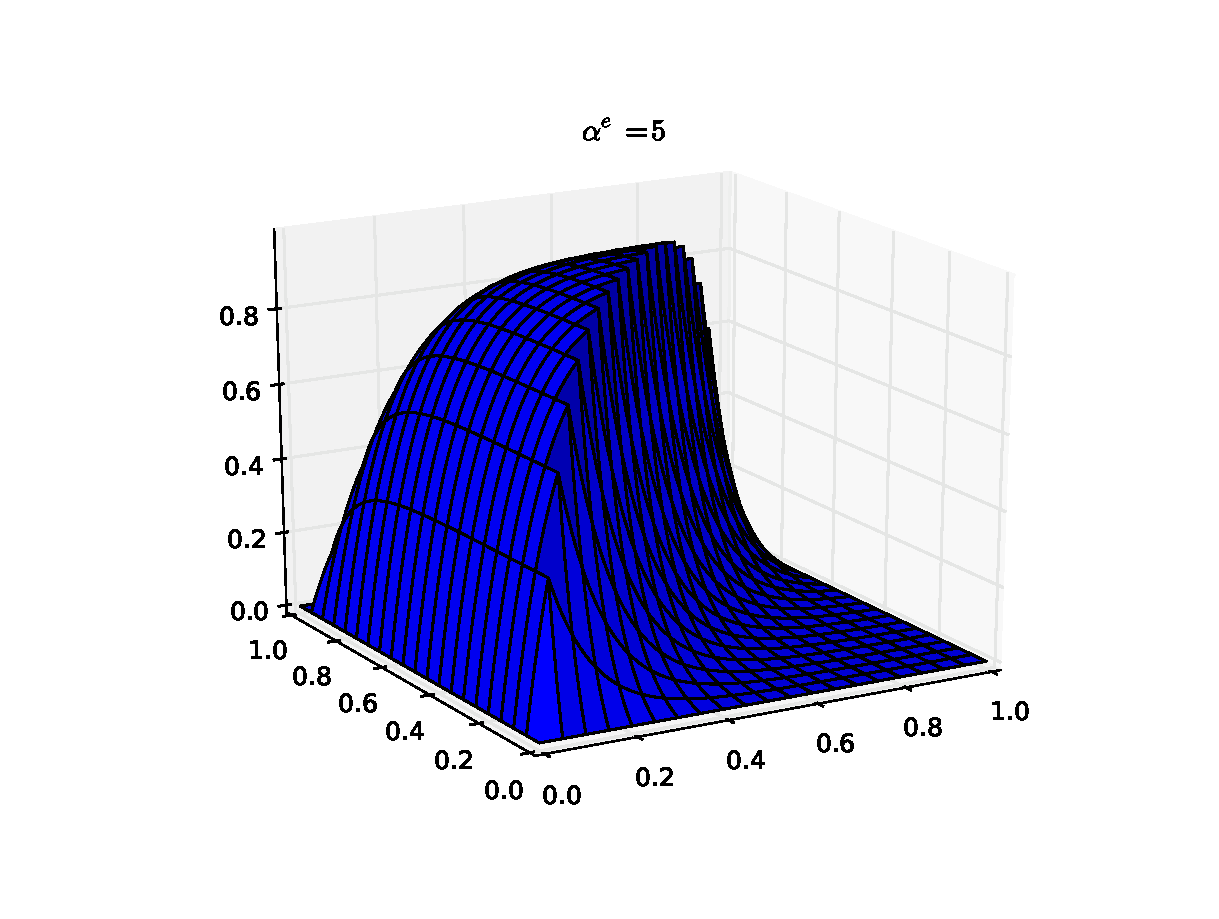
\includegraphics[width=0.45\textwidth]{surf5e0.pdf}
% }}
% \mbox{\subfigure{
% 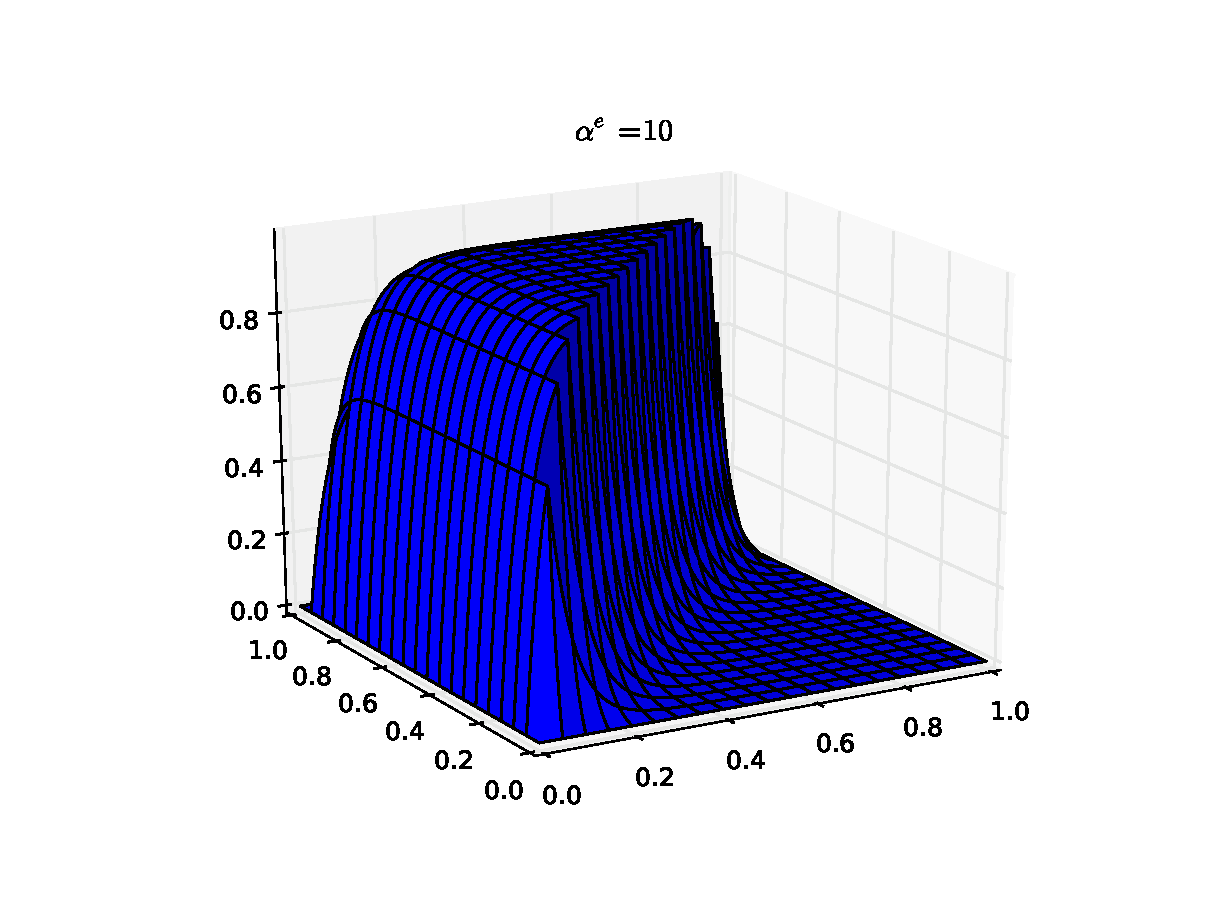
\includegraphics[width=0.45\textwidth]{surf1e1.pdf}
% }
% \subfigure{
% 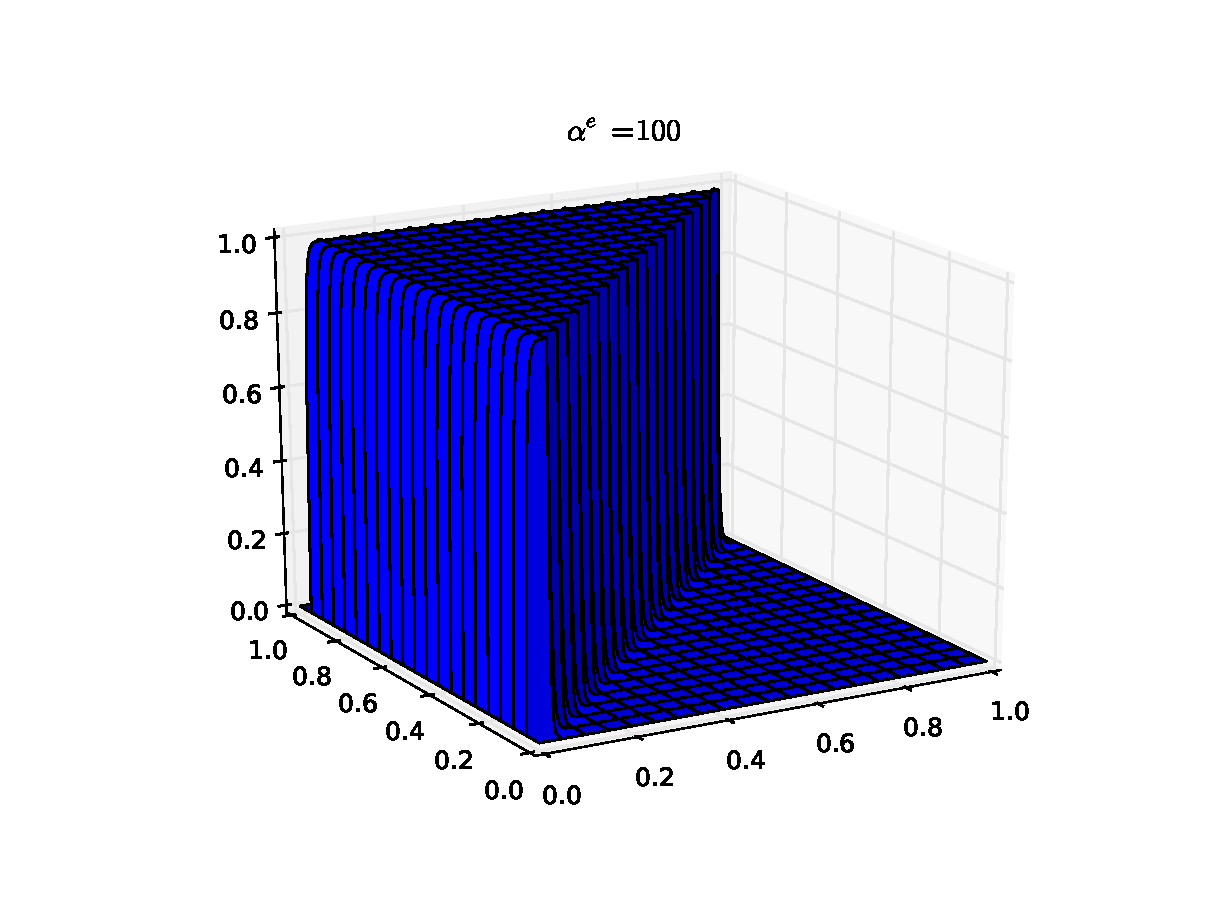
\includegraphics[width=0.45\textwidth]{surf1e2.pdf}
% }}
% \caption{Element Green's function for the one-dimensional advection-diffusion}
% \end{figure}

\clearpage
\newpage

\section*{Problem 8.2}
Plots of residual free bubbles for $u=h^e=1$.
\begin{figure}[h!]
\centering
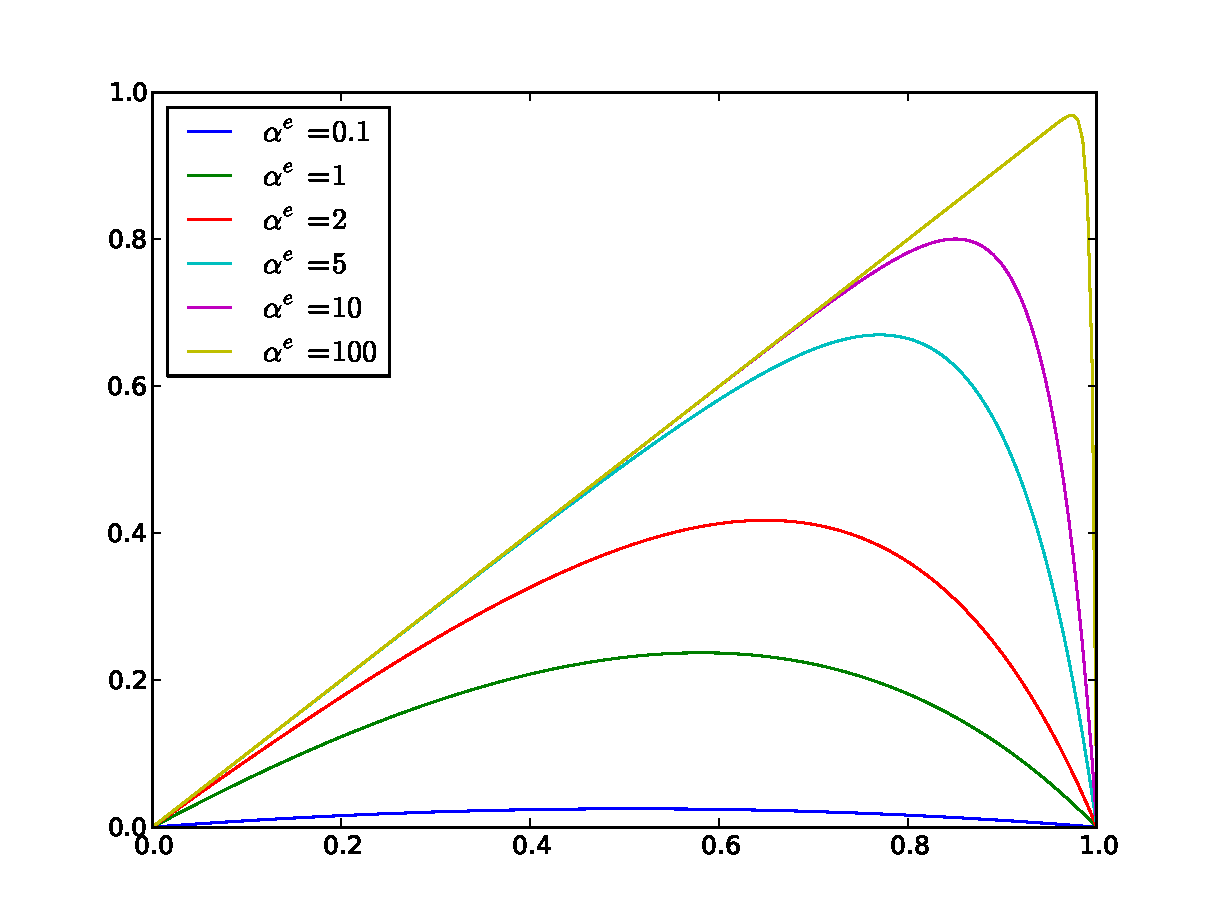
\includegraphics[width=0.8\textwidth]{bubbles.pdf}
\end{figure}

\end{document}

